El \ac{SW} de \ac{S1} se ha desarrollado íntegramente usando el lenguaje Python y los editores de código Visual Studio Code y PyCharm.

Es de vital importancia destacar que el \ac{SW} de \ac{S1} esta formado por dos secciones diferenciadas: código de la interfaz gráfica de usuario (GUI) y código que gestiona la lógica de las comunicaciones entre \ac{S1} y \ac{S2}.

Puesto que esta división se considera esencial, cada una de las secciones del código de \ac{S1} será descrita en detalle de forma independiente en los apartados siguientes.

\subsection{Interfaz Gráfica de Usuario (GUI)}

La interfaz gráfica de usuario ha sido desarrollada haciendo uso de la biblioteca gráfica multiplataforma \textit{Qt}, la cual se encuentra originalmente implementada en $C++$ y que ha sido adaptada a Python, siendo conocida también como \textit{PyQt}. Esta librería gráfica permite un desarrollo rápido y sencillo de interfaces gráficas de usuario mediante el paradigma de programación orientada a objetos.

En primer lugar, es importante destacar las principales razones que han desembocado en la elección de esta librería:
\begin{itemize}
    \item La curva de aprendizaje de esta librería es rápida y permite desarrollar interfaces gráficas de forma ágil y eficaz.
    \item La librería dispone de abundante documentación, la cual facilita su uso en el proyecto.
    \item Qt cuenta con una gran variedad de componentes gráficos y herramientas, las cuales cubren de sobra las aspiraciones de este proyecto.
    \item Es una de las librerías gráficas mas usadas por la comunidad de desarrolladores en la programación de interfaces gráficas empleando Python.
    \item Proporciona una herramienta de diseño gráfico de interfaces de usuario llamada \textit{Qt Designer} y que agiliza las etapas tempranas de desarrollo de la interfaz gráfica, sobre todo en cuanto al ámbito de la distribución gráfica de los distintos \textit{widgets}, botones, desplegables, etc. Este archivo XML puede ser cargado desde el código Python y por lo tanto, cada componente gráfico se corresponde con un objeto.
\end{itemize}

Una vez se ha introducido la librería gráfica utilizada, se procede a describir la interfaz gráfica desarrollada, las decisiones tomadas durante este desarrollo y el resultado final obtenido.

En términos generales, la interfaz gráfica de usuario se considera un componente esencial del proyecto y su función es la de facilitar la interacción entre el usuario y el brazo robótico. Tal y como se ha podido ver en apartados anteriores de esta memoria, la interfaz gráfica de usuario ofrece una al usuario la posibilidad de:
\begin{itemize}
    \item Controlar el movimiento del brazo robótico mediante el control de algunos parámetros del mismo, por ejemplo, mediante la posición angular de los servomotores o la posición cartesiana del \textit{end-effector} del brazo.
    \item Visualizar gráficamente una previsualización de la posición del brazo antes de que el mismo realice el movimiento físicamente.
    \item Gestionar la comunicación de \ac{S1} y \ac{S2} a través de la selección de un puerto serie.
    \item Mostrar información sobre la ejecución de la aplicación y el estado del sistema.
\end{itemize}

En relación a lo anteriormente mencionado, se planteó un diseño teórico que aproximaba la apariencia de la interfaz gráfica de usuario según los requisitos planteados:

\begin{figure}[H]
    \centering
    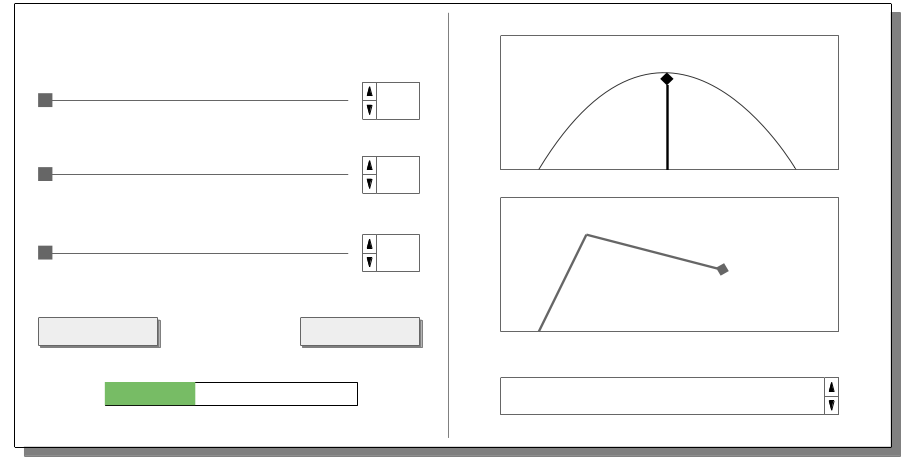
\includegraphics[width=0.6\linewidth]{RS/images/InterfaceSketch-MkII.png}
    \caption{Diseño propuesto para la interfaz gráfica de usuario.}
    \label{fig:ui_design}
\end{figure}

En el diseño anterior se pueden identificar algunos elementos cruciales que deben trasladarse inequívocamente a la interfaz gráfica de usuario final:
\begin{itemize}
    \item \textit{Sliders} que permitan al usuario visualizar y modificar los valores de las coordenadas angulares de los motores, así como de las coordenadas cartesianas del \textit{end-effector}
    
    \item \textit{SpinBoxes} que permitan al usuario visualizar y modificar el valor numérico representado por el \textit{Slider}
    
    \item Botones que permitan al usuario ejecutar un movimiento, así como seleccionar el tipo de control de los parámetros del brazo (ángulos de giro o posición cartesiana)
    
    \item Representaciones gráficas de la posición del brazo robótico tras realizar un movimiento generado por el usuario.
    
    \item Una barra de progreso que muestre el estado del movimiento que está realizando el brazo robótico.
    
    \item Una consola que muestre los \textit{logs} que genera la aplicación del sistema \ac{S1}
\end{itemize}

Teniendo el cuenta el diseño teórico propuesto previamente a desarrollar la interfaz gráfica de usuario, se procede a implementar dicho diseño utilizando la herramienta \textit{Qt Designer}:

\begin{figure}[H]
    \centering
    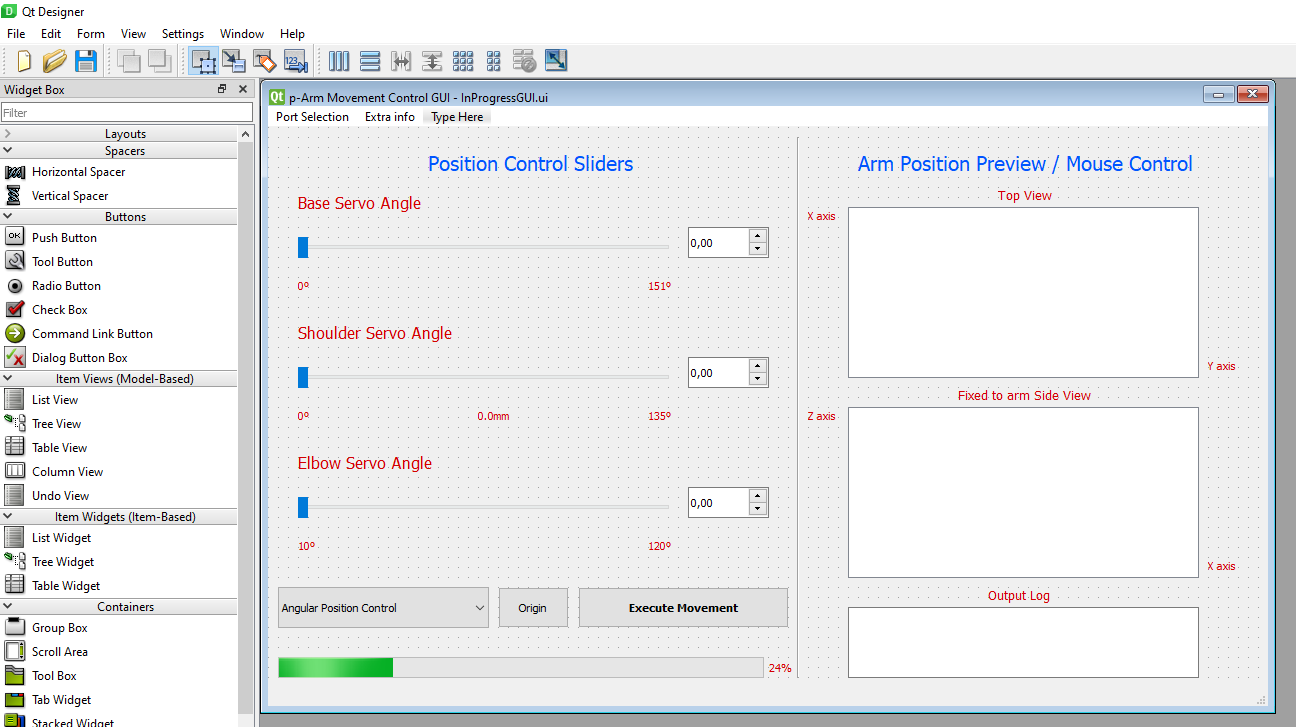
\includegraphics[width=0.8\linewidth]{pictures/DesignerGui.PNG}
    \caption{Diseño final para la interfaz gráfica de usuario.}
    \label{fig:ui_QtDesigner}
\end{figure}

Mediante la herramienta anterior, se puede diseñar gráficamente cual va a ser la apariencia de la interfaz gráfica. Tal y como se puede ver en la parte izquierda de la imagen, Qt proporciona numerosos componentes gráficos de todos los tipos, los cuales, pueden ser incluidos en el diseño con tan solo arrastrarlos al mismo. Esta herramienta de diseño, proporciona un archivo de salida XML que tiene extensión .ui y que posteriormente será cargado desde Python para la programación de la lógica que existe entre los distintos componentes gráficos.

\begin{figure}[H]
    \centering
    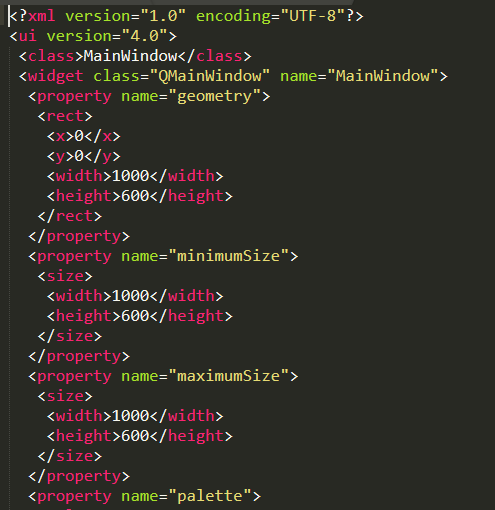
\includegraphics[width=0.55\linewidth]{pictures/XmlGui.PNG}
    \caption{Fragmento del archivo XML que describe la apariencia de la GUI.}
    \label{fig:ui_XML}
\end{figure}

A continuación se presenta una breve descripción de los componentes gráficos que aparecen en el diseño final de la interfaz gráfica de usuario y que posteriormente será extendida para mostrar los detalles técnicos mas relevantes:
\begin{itemize}
    \item Por un lado, en la sección izquierda de la interfaz gráfica de usuario se encuentran los siguientes componentes:
    \begin{itemize}
        \item En la barra de herramientas de la parte superior se encuentran el menú desplegable de selección de puerto serie, así como el menú desplegable que da a conocer la documentación del proyecto al usuario.
        \item En la parte central, tal y como describe el título ``\textit{Position Control Sliders}'', se encuentran los \textit{Sliders} y \textit{SpinBoxes} que permiten al usuario controlar el valor de las coordenadas angulares de los motores y las coordenadas cartesianas del \textit{end-effector}.
        \item Justo debajo de los \textit{Sliders}, se encuentran tres botones que permiten al usuario: cambiar el tipo de coordenadas de los \textit{Sliders}, devolver al brazo robótico a su posición inicial y ejecutar o cancelar un movimiento.
        \item En la parte mas inferior de la mitad izquierda, se encuentra la barra de progreso que indica el estado del movimiento en el momento de la realización del mismo.
    \end{itemize}
    \item Por otro lado, en la sección derecha de la interfaz gráfica de usuario se encuentran lo siguientes componentes:
    \begin{itemize}
        \item Tal y como describe el título, en esta parte de la interfaz se encuentran las dos representaciones gráficas de la posición del brazo robótico, las cuales además, permiten al usuario controlar la posición del brazo mediante movimientos del ratón.
        \item Justo debajo de ambas representaciones, se encuentra la consola de salida que proporciona al usuario la información sobre los \textit{logs} generados por la aplicación.
    \end{itemize}
\end{itemize}

En relación a los componentes gráficos anteriores, es importante destacar algunas decisiones esenciales que han sido tomadas durante el desarrollo de la interfaz gráfica y que por lo tanto han condicionado el resultado final:

En primer lugar, inicialmente se disponía de unos rangos de valor teóricos para cada uno de los \textit{Sliders} y \textit{SpinBoxes}, los cuales, tras realizar algunas pruebas físicas con el prototipo del brazo robótico, han sido reajustados para cumplir con las limitaciones físicas y de seguridad de la estructura:
    \begin{itemize}
        \item Cuando los controles se encuentran en modo de coordenadas angulares, los tres \textit{Sliders} y \textit{SpinBoxes} representan a los ángulos de giro $(\theta_{0}, \theta_{1}, \theta_{2})$. Estos ángulos tienen los siguientes rangos de valores:
        \begin{itemize}
            \item El ángulo $\theta_{0}$ es ajustable entre 0° y 151°, que coincide con el rango de giro máximo del servomotor de la base.
            \item El ángulo $\theta_{1}$ es ajustable entre 0° y 135°, este rango se deduce de las limitaciones físicas de la estructura del brazo.
            \item El ángulo $\theta_{2}$ es ajustable entre 10° y 120°, este rango se deduce de las limitaciones físicas de la estructura del brazo.
        \end{itemize}
        \begin{figure}[H]
            \centering
            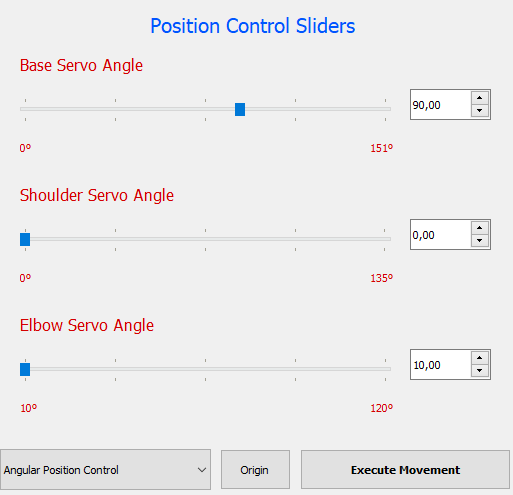
\includegraphics[width=0.55\linewidth]{pictures/Joints_Gui.PNG}
            \caption{Controles en modo coordenadas angulares.}
            \label{fig:ui_joint}
         \end{figure}
        \item Cuando los controles se encuentran en modo de coordenadas cartesianas, los tres \textit{Sliders} y \textit{SpinBoxes} representan a la posición cartesiana del \textit{end-effector} del brazo $(x, y, z)$. Estas coordenadas tienen los siguientes rangos de valores:
        \begin{itemize}
            \item La coordenada X es ajustable entre 0.0mm y 346.0mm, puesto que el \textit{end-effector} siempre se sitúa delante de la base, coincidiendo con la parte positiva del eje X. 
            \item La coordenada Y es ajustable entre -346.0mm y 346.0mm, puesto que el \textit{end-effector} puede desplazarse hacia la derecha e izquierda de la base, coincidiendo con la parte positiva y negativa del eje Y.
            \item La coordenada Z es ajustable entre -106.0mm y 360.6mm, puesto que el \textit{end-effector} puede desplazarse hacia arriba y abajo, teniendo como limite inferior la parte mas baja de la base del brazo y coincidiendo con la parte positiva  y negativa del eje Z.
        \end{itemize}
        \begin{figure}[H]
            \centering
            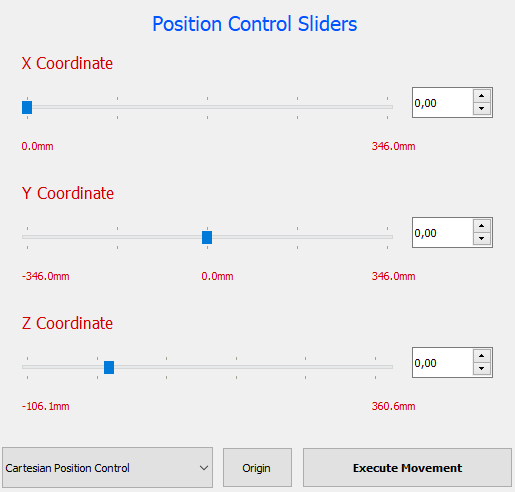
\includegraphics[width=0.55\linewidth]{pictures/Cartesian_Gui.PNG}
            \caption{Controles en modo coordenadas cartesianas.}
            \label{fig:ui_cartesian}
        \end{figure}
    \end{itemize}

En segundo lugar y en relación con las representaciones gráficas del brazo robótico, se ha tomado la decisión de incluir dos vistas:
    \begin{itemize}
        \item Vista cenital o desde arriba: la cual muestra como el ángulo $\theta_{0}$ o las coordenadas X e Y afectan a la posición del brazo. Esta vista es absoluta y no se encuentra fijada a la estructura del brazo robótico.
        \item Vista lateral o de perfil fijada: la cual muestra como los ángulos $\theta_{1}$ y $\theta_{2}$ o las coordenadas X, Y, Z afectan a la posición del brazo. Esta vista cuenta con una particularidad y es que se encuentra fijada a la estructura del robot y por lo tanto, no contempla el desplazamiento de profundidad del brazo robótico, es decir, el enfoque es siempre completamente paralelo al lateral del brazo. 
        \item En ambas vistas se muestran los dos segmentos del brazo en colores distintos para  así distinguirlos con claridad, así como la base sobre la que se encuentra situado el brazo.
         \item Ambas representaciones gráficas anteriores usan los modelos matemáticos de cinemática directa e inversa para realizar los cálculos que permiten dibujar los diferentes puntos y segmentos.
        \begin{figure}[H]
            \centering
            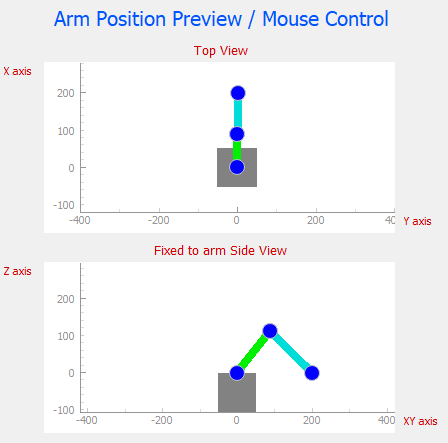
\includegraphics[width=0.55\linewidth]{pictures/Views_GUI.PNG}
            \caption{Representaciones gráficas de la posición del brazo.}
            \label{fig:ui_views}
         \end{figure}
    \end{itemize}
    
Cabe destacar que, a pesar de que los controles del brazo pueden ser ajustados libremente por el usuario, se tiene que el brazo robótico tiene un rango limitado por su estructura física y por ello, se ha programado un método que verifica si la posición que el usuario ha seleccionado es viable. En caso de serlo, el movimiento puede ser ejecutado y enviado como orden a \ac{S2}, en caso contrario, la representación del brazo se colorea de color rojo y el botón de ejecutar movimiento se desactiva, de esta forma el usuario es notificado y debe modificar los valores de los controles.    

Continuando con el proceso de desarrollo de la interfaz gráfica de usuario y una vez se ha creado el diseño gráfico de la misma, el siguiente paso consiste en la programación de la lógica que existe entre los diferentes componentes gráficos, así como sus interacciones. Para la programación de la lógica entre los componentes gráficos, se hace uso de las señales que proporciona la librería Qt.

En la librería gráfica Qt, las señales representan el mecanismo principal para notificar cambios de estado y eventos que afectan a componentes gráficos de una interfaz. El concepto de señal, puede ser asemejado con el concepto de interrupción, en el cual, cuando sucede cierto evento, se dispara una señal  o notificación que puede ser manejada por el programador y que dispara la realización de una cierta rutina. Uno de los ejemplos mas claros de este mecanismo, es la señal ``\textit{clicked()}'' de un botón del tipo ``\textit{QPushButton}'' perteneciente a los \textit{widget} que ofrece Qt: cuando el botón es clickado, se dispara una señal que  permite al usuario ejecutar una función programada por el mismo tras este evento. 

El concepto mas importante tras las señales es el hecho de que Qt ofrece la posibilidad de conectar cada una de las  posibles señales a la  ejecución de un método programado por el desarrollador, de esta forma, mediante estas señales, se puede establecer una lógica que orquesta las interacciones entre los diferentes componentes gráficos.

Teniendo en cuenta el concepto anterior, el código de la interfaz gráfica de usuario consiste en un archivo Python desde el cual se carga el archivo XML que contiene el diseño gráfico de la interfaz, y en el cual se han programado los diferentes métodos a ejecutar tras la recepción de las diferentes señales de los distintos componentes gráficos.

Como detalle final, es importante remarcar que el punto de enlace entre el código de la interfaz gráfica y el código de la lógica de comunicaciones se realiza mediante la clase denominada  ``\textit{control interface}'', la cual describe en el subapartado siguiente. Esta clase proporciona una serie de métodos que al ser ejecutados dentro de las rutinas de gestión de señales, disparan y ejecutan los métodos necesarios del código de la lógica de comunicaciones que permiten el envío de las ordenes generadas por el usuario mediante la interfaz gráfica.

Finalmente se muestra una imagen de la interfaz gráfica de usuario final en ejecución:
\begin{figure}[H]
    \centering
    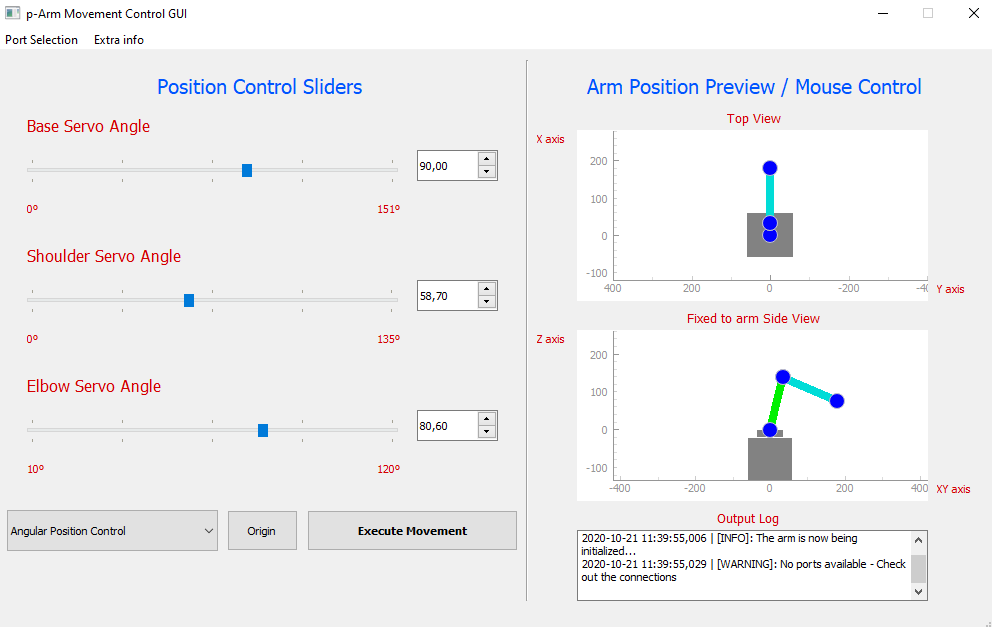
\includegraphics[width=0.85\linewidth]{pictures/Gui_Final.png}
    \caption{Interfaz de usuario final en ejecución}
    \label{fig:ui_finalexe}
\end{figure}

El código de la interfaz gráfica de usuario se muestra en el anexo y el archivo que lo contiene recibe el nombre de ``GUI.py''.


\subsection{Lógica de comunicaciones}
Antes de proceder con la explicación del código conviene especificar ciertos aspectos destacados del \ac{SW}.

Al tener que comunicar \ac{S1} con \ac{S2}, es necesario que existan hilos de cómputo dedicados específicamente a las labores de lectura y escritura en la UART. Esto se debe a que no se debe ocupar el hilo principal de cómputo con labores de comunicación ya que esto supondría bloquear la interacción con la interfaz gráfica mientras duren las comunicaciones.
Por otro lado, es necesario un hilo especial para poder interactuar con uno de los elemento de la interfaz desde el hilo de comunicación.

Ante esta circunstancia se ha decidido que el \ac{SW} se ejecutará en hasta 4 hilos de cómputo distintos y concurrentes.

Dichos hilos son:

\begin{itemize}
    \item El hilo principal: en el se ejecuta la interfaz gráfica y la lógica de control siempre y cuando esta no suponga una comunicación con el \ac{S2}.
    \item Hilos dedicados a comunicación: estos hilos se crean bajo demanda al iniciarse una comunicación con \ac{S2} y se destruyen tras terminar su labor. Gracias a estos hilos, la interfaz gráfica puede seguir ejecutándose en el hilo principal.
    \item Hilo dedicado al demonio de pulsos: este hilo se crea tras realizarse la sincronización inicial. Su cometido es mandar mensajes periódicos a través de la UART para indicarle a \ac{S2} que \ac{S1} aún sigue conectado y que no se ha desconectado.
    \item Hilo dedicado a la actualización de la barra de progreso: este hilo se encarga de actualizar la barra de progreso que representa el porcentaje del movimiento que ya se ha realizado, creándose en el hilo de comunicación. El motivo por el cual es necesario actualizarlo desde un hilo distinto al principal es que solo \ac{S2} conoce cuánto tiempo tardará en realizarse el movimiento y, dado que el hilo principal no puede acceder a este dato hasta que el futuro acabe, es necesario que la interacción se haga desde un hilo que pueda acceder al dato de manera independiente e inmediata.
\end{itemize}

El modelo de comunicación asíncrona plantea ciertos problemas.

Uno de ellos es el acceso concurrente a recursos. Esto se puede observar en el acceso al canal de comunicaciones. El hilo demonio escribe de manera periódica en el canal de comunicación un mensaje, el cual sirve de pulso. Puede ocurrir que, de manera concurrente, sea necesario que un hilo de comunicación envíe una orden de movimiento a \ac{S2}.

Si el planificador de tareas del sistema operativo expulsa uno de los hilos en mitad de la comunicación y da paso al otro, los dos mensajes se mezclarían originando un fallo en la comunicación. 

Para evitar esta situación, el acceso a la UART es bloqueado siempre que un hilo accede a este recurso y no se desbloquea hasta que el hilo ha terminado la comunicación.

Otro problema es la comunicación de mensajes entre hilos y la sincronización de recepción y envió de estos. 

Este problema se origina ante la necesidad de que la interfaz gráfica se mantenga actualizada con los datos que se reciben en el hilo de comunicación. Para solucionarlo se han empleado futuros, los cuales pueden desencadenar la ejecución de una función en el hilo principal, cuando el futuro finaliza su ejecución.

Concretamente, el futuro que se ha implementado en \ac{S1} se encarga de ordenar el movimiento del brazo, monitorizarlo, recoger posibles errores, pedir las posiciones reales al acabar el movimiento y finalmente comunicarle dichas posiciones a la interfaz gráfica cuando esta las requiera.

%% INDICAR PREVIAMENTE QUE PUEDE DEVOLVER O BIEN EL ERROR QUE SE HAYA RECOGIDO
%% O BIEN LA INTERFAZ DE 'CONTROL' EN SÍ CON LAS POSICIONES ACTUALIZADAS
Además, el futuro puede contener los datos que la interfaz principal necesita y por tanto esta puede acceder a ellos.

%% UNIR CON LO DE ARRIBA PORQUE ES XD (SEGÚN MIHAI)

La lógica de control se ha dividido en varios paquetes para encapsular distintas funcionalidades del sistema por separado, estos paquetes son: ``\texttt{communications}'', ``\texttt{control}'', ``\texttt{gcode}'', ``\texttt{logger}'', ``\texttt{security}'' y ``\texttt{utils}''.

A continuación se procede a explicar la funcionalidad de cada uno de los paquetes a un nivel de abstracción alto, junto con una explicación más detallada de cada uno de los ficheros \texttt{.py}.

Además de las explicaciones dadas en esta sección, existen comentarios en el código que concretizan el funcionamiento de cada una de las funciones contenidas dentro de los distintos ficheros \texttt{.py}.

A continuación se procede a explicar cada uno de los paquetes.

\subsubsection{\texttt{communications}}
Este paquete gestiona las comunicaciones desde y hacia \ac{S1}. Su principal cometido es facilitar la operación y la lectura del búfer de recepción junto con la escritura por un puerto UART.

Contiene un único fichero, ``\texttt{connection.py}'' (anexo \ref{lst:connection_py}), en el cual están definidas todas las funciones relacionadas con la lectura y la escritura a través del puerto UART.

Es aquí donde, mediante el uso de cierres de exclusión mutua, se consigue que el acceso a la UART se haga de manera individual por parte de los procesos.

Cabe destacar que para poder utilizar este puerto para la comunicación se ha hecho uso de la librería ``\texttt{pyserial}''\footnote{\url{https://pypi.org/project/pyserial/}} de Python.

También se ha empleado la librería ``\texttt{threading}'' la cual de acceso a los cierres de exclusión mutua, llamados \textit{locks} en dicha librería.

\subsubsection{\texttt{control}}

Este paquete contiene la lógica de control propiamente dicha. Sirve para implementar los métodos principales de movimiento, de gestión de la comunicación, de creación del demonio de pulsos y de  sincronización inicial. Además, ofrece una interfaz lógica para que la interfaz de usuario pueda, a través de los botones que aparecen en pantalla, comunicarse con la lógica de control.

El paquete está conformado por 4 archivos:

\begin{itemize}
    \item \texttt{control.py}(anexo \ref{lst:control_py}): el cual implementa los métodos de movimiento y petición de posiciones además del método que desencadena el proceso de sincronización inicial. Es el archivo principal de control y sus funciones desencadenan llamadas a todos los demás paquetes para poder realizar funciones complejas.
    \item \texttt{control\_interface.py}(anexo \ref{lst:control_interface_py}): es una interfaz que implementa parte de los métodos de control.py. Este archivo es utilizado por la GUI para poder desencadenar acciones en \ac{S1} a partir de la interacción del operario con la interfaz gráfica.
    \item \texttt{control\_management.py}(anexo \ref{lst:control_management.py}): ofrece funciones auxiliares que permiten a control.py monitorizar que las órdenes enviadas a \ac{S2} son realizadas con éxito o, en caso contrario, controlar los errores que se pudieran producir.
    Además, aquí se encuentran las funciones que hacen peticiones a \ac{S2}.
    \item \texttt{\textit{heart\_beat}(anexo \ref{lst:heart_beat.py})}: ofrece funciones que permiten la instanciación de un objeto el cual envía un mensaje de manera periódica a través de la UART.
\end{itemize}

Cabe destacar que en este paquete se han utilizado librerías  que implementan el uso de futuros en Python con el objetivo de poder monitorizar el movimiento de \ac{S2} sin necesidad de bloquear la interfaz de usuario.

\subsubsection{\texttt{gcode}}

Aquí se encuentran la lógica de interpretación y generación de las tramas de GCODE que se transmiten entre \ac{S1} y \ac{S2}.

Contiene 2 ficheros:

\begin{itemize}
    \item \texttt{generator.py}(anexo \ref{lst:generator_py}): este archivo contiene las funciones que, a partir de los valores que reciben como parámetros, generan las tramas en el formato adecuado para ser enviadas.
    
    \item \texttt{interpreter.py}(anexo \ref{lst:interpreter_py}): analizador gramático de los \textit{bytes} que hay en el búfer de \ac{S1}.
    Para poder realizar esta labor, transforma los \textit{bytes} en cadena de caracteres y posteriormente analiza dichas cadenas y las interpreta.
\end{itemize}

Se ha usado la librería ``typing'' para simplificar el tratamiento de los datos y la interpretación de las tramas.

\subsubsection{\texttt{logger}}

Este paquete permite llevar un registro de los datos y las acciones importantes que ocurren en \ac{S1}. Genera un archivo en el que se guardan diferentes datos para poder hacer \textit{debugging} y revisar \textit{crashlogs}.
Destaca el uso de la librería ``\texttt{logging}'' para poder generar registros de manera unificada y poder definir distintos niveles dentro de los registros, de manera que se pueden definir
niveles que serán ignorados.

Contiene dos ficheros, \texttt{logger.py} (anexo \ref{lst:logger_py}), el cual alberga las funciones necesarias para crear el archivo y operar con él, además de dar un formato estándar a las diferentes trazas;
y el fichero \texttt{PyQtHandler.py} (anexo \ref{lst:pyqthandler_py}), el cual
contiene un \textit{wrapper} para que la librería \texttt{logging} también escriba
los registros en la interfaz de usuario, en un \textit{widget} de Qt.

\subsubsection{\texttt{security}}

A través de este paquete, \ac{S1} consigue autenticar al sistema \ac{S2} y viceversa.

Contiene un solo archivo, \texttt{rsa.py}(anexo \ref{lst:rsa_py}), el cual alberga las funciones necesarias para que, a partir de los números procedentes de \ac{S2}, se pueda autenticar al emisor desde la trama recibida y poder reenviarla encriptada posteriormente.

Se ha usado la librería ``typing'' para simplificar el tratamiento de los datos y la interpretación de las tramas.

\subsubsection{\texttt{utils}}

En este paquete se encuentran todos los archivos auxiliares que no se puedan ubicar en ningún otro paquete.

%% INSERTAR REFERENCIA AL FICHERO \ref{lst:---}
Solo contiene un archivo, \texttt{error\_data.py}(anexo \ref{lst: error_data.py}), el cual simplemente implementa un tipo de dato creado especialmente para poder contener de una manera más organizada los datos referentes a los errores provenientes de \ac{S2}.

Se emplea la librería \texttt{collections} para permitir el uso de tipos de datos auxiliares.

Por otra parte, se declara una nueva estructura de datos en el fichero \texttt{atomics.py}
(listado de código \ref{lst:atomics_py}). Se define una clase base 
\lstinline[style=Python]!class Atomic(ABC, Generic[T])! que se diseña para que las clases
hijas hereden de ella y establezcan el tipo de dato que van a contener, junto con
las especializaciones requeridas.

Se definen dos clases hijas:
\begin{itemize}
    \item \lstinline[style=Python]!class AtomicFloat(Atomic[float])! para contener
    valores en coma flotante de forma atómica.
    \item \lstinline[style=Python]!class AtomicInteger(Atomic[int])! para contener
    valores enteros y añadir además opciones para incrementar dicho valor.
\end{itemize}

La principal función de estas clases no es solo guardar un dato de forma atómica
sino además poder utilizar la misma dirección de memoria a lo largo del programa,
pudiendo tener acceso simultáneo al recurso.